% !TEX root = ./arock_pkg_main.tex
\subsection{Nonnegative Matrix Factorization}

We consider the following Nonnegative Matrix Factorization problem

\begin{equation*}
	\Min_{X \geq 0,Y \geq 0} ~||A-X^T Y||_2^2,
\end{equation*}
where $A \in \RR^{m\times n}$, $X \in \RR^{k \times m}$ and $Y \in \RR^{k \times m}$.
This problem, despite being nonconvex has a special form.
The objecctive function  is block multiconvex\footnote{the objective function is convex when all but a few specific variables are held fixed} and it's reguralizers are separable.
Recent work by Davis (insert citation) has shown that this type of problem can be solved asynchronously.
As the problem is nonconvex, convergence is given to a local minimizer, not a global minimizer.

We run MOTAC on a synthetic problem, $A=\hat X^T \hat Y$ ,  with $m=1000$ and $k=20$.
Elements of $\hat X$ and $\hat Y$ sampled independently from $N(0, 1)$ normal distribution, then thresholded positive.
We ran the tests with variable number of threads and iterations. 
The following results are the averages resulting from 20 runs.


\begin{figure}[!h]
        \centering
       \begin{subfigure}[b]{0.4\textwidth}
                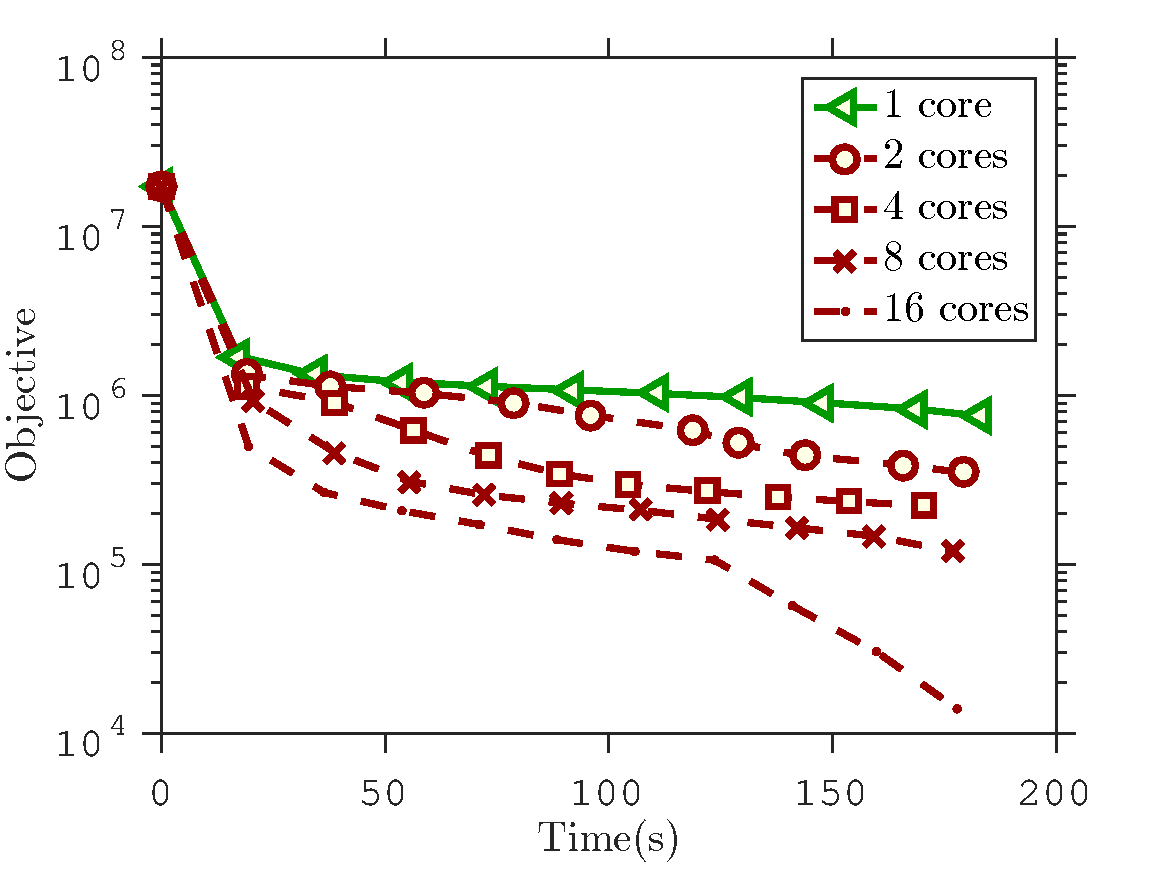
\includegraphics[width=\textwidth]{./figs/NMF_plot}
                \caption{Objective vs walll clock time}
        \end{subfigure}
        ~~
        \begin{subfigure}[b]{0.4\textwidth}
                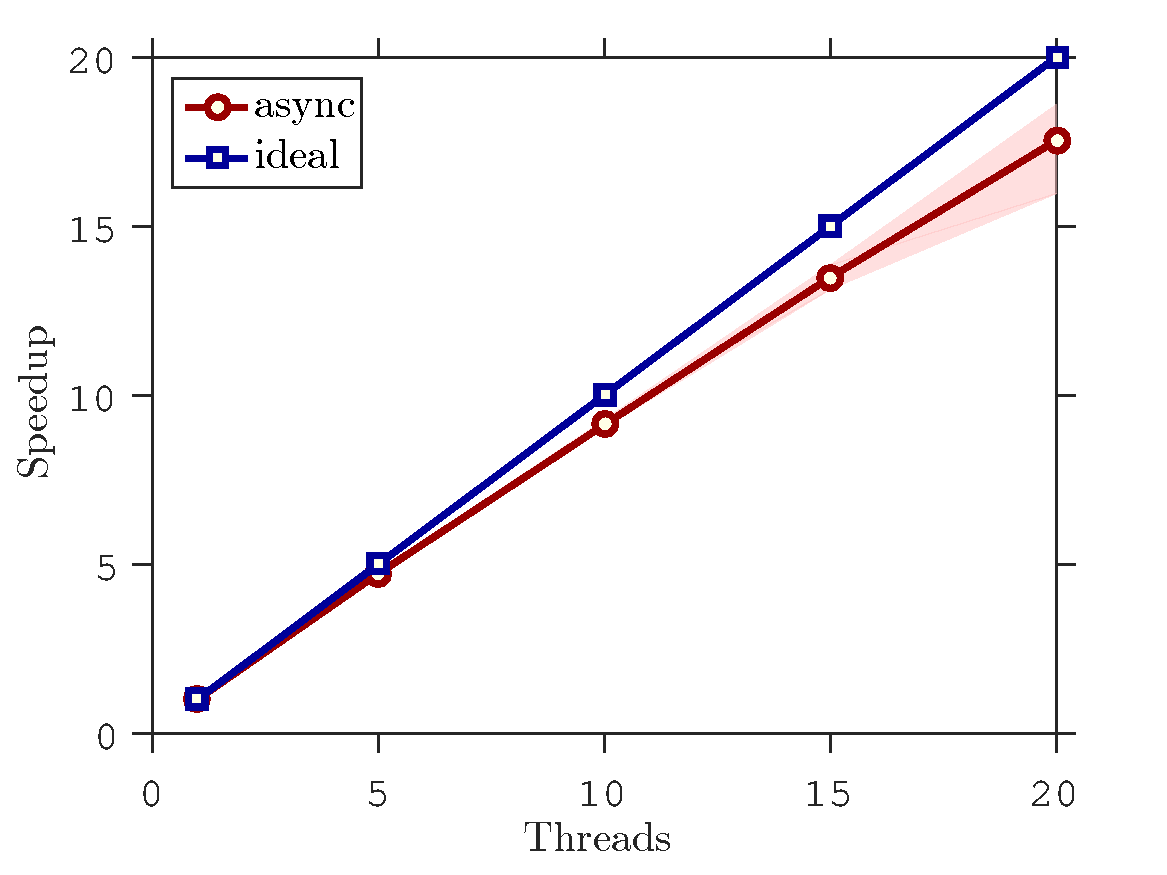
\includegraphics[width=\textwidth]{./figs/speedup}
                \caption{speedup}
        \end{subfigure} 
        \caption{NMF results}\label{fig:NMF_speedup}
\end{figure}


To show scalability we increased the dimension of $k$, and tested the speedup.
\begin{table}[!hb]
\centering
\begin{tabular}{rrrr}
 \toprule
{threads}&{k=10}&{k=20}&{k=100}\\\cmidrule{1-4}
1&1.00&1.00&1.00\\%\hline
2&1.97&1.98&1.98\\%\hline
4&3.75&3.75&3.76\\%\hline
8&7.12&7.33&7.35\\%\hline
16&13.38&14.51&14.43\\%\hline
\bottomrule
\end{tabular}
 \caption{\label{tab:nmf_res}Speedup results for nonnegative matrix factorization. }                  
\end{table}